\begin{figure}[h]
\centering
\tikzset{every picture/.style={line width=0.75pt}} %set default line width to 0.75pt        
\resizebox{11cm}{6cm}{

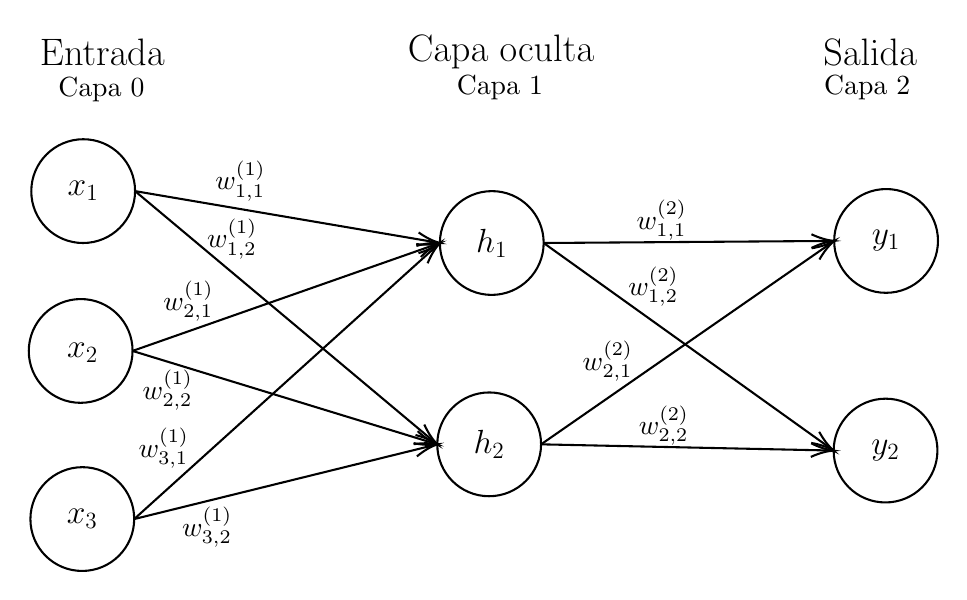
\begin{tikzpicture}[x=0.75pt,y=0.75pt,yscale=-1,xscale=1]
%uncomment if require: \path (0,398); %set diagram left start at 0, and has height of 398

%Shape: Circle [id:dp014797891854668621] 
\draw   (44.21,86) .. controls (44.24,72.19) and (55.46,61) .. (69.27,61) .. controls (83.08,61) and (94.24,72.19) .. (94.21,86) .. controls (94.17,99.81) and (82.95,111) .. (69.14,111) .. controls (55.33,111) and (44.17,99.81) .. (44.21,86) -- cycle ;
%Shape: Circle [id:dp058244464473876545] 
\draw   (43,163) .. controls (43.04,149.19) and (54.26,138) .. (68.07,138) .. controls (81.88,138) and (93.04,149.19) .. (93,163) .. controls (92.97,176.81) and (81.75,188) .. (67.94,188) .. controls (54.13,188) and (42.97,176.81) .. (43,163) -- cycle ;
%Shape: Circle [id:dp31737473014049844] 
\draw   (43.79,244) .. controls (43.83,230.19) and (55.05,219) .. (68.86,219) .. controls (82.67,219) and (93.83,230.19) .. (93.79,244) .. controls (93.76,257.81) and (82.53,269) .. (68.73,269) .. controls (54.92,269) and (43.76,257.81) .. (43.79,244) -- cycle ;
%Shape: Circle [id:dp014201185840476138] 
\draw   (431.05,110) .. controls (431.09,96.19) and (442.31,85) .. (456.12,85) .. controls (469.93,85) and (481.09,96.19) .. (481.05,110) .. controls (481.02,123.81) and (469.8,135) .. (455.99,135) .. controls (442.18,135) and (431.02,123.81) .. (431.05,110) -- cycle ;
%Shape: Circle [id:dp7248329472734] 
\draw   (430.79,211) .. controls (430.83,197.19) and (442.05,186) .. (455.86,186) .. controls (469.66,186) and (480.83,197.19) .. (480.79,211) .. controls (480.75,224.81) and (469.53,236) .. (455.72,236) .. controls (441.92,236) and (430.75,224.81) .. (430.79,211) -- cycle ;
%Straight Lines [id:da23388739067292408] 
\draw    (93,163) -- (239.18,111.66) ;
\draw [shift={(241.07,111)}, rotate = 520.65] [color={rgb, 255:red, 0; green, 0; blue, 0 }  ][line width=0.75]    (10.93,-3.29) .. controls (6.95,-1.4) and (3.31,-0.3) .. (0,0) .. controls (3.31,0.3) and (6.95,1.4) .. (10.93,3.29)   ;

%Straight Lines [id:da46924522998984264] 
\draw    (93.79,244) -- (239.59,112.34) ;
\draw [shift={(241.07,111)}, rotate = 497.92] [color={rgb, 255:red, 0; green, 0; blue, 0 }  ][line width=0.75]    (10.93,-3.29) .. controls (6.95,-1.4) and (3.31,-0.3) .. (0,0) .. controls (3.31,0.3) and (6.95,1.4) .. (10.93,3.29)   ;

%Straight Lines [id:da5852104107316262] 
\draw    (94.21,86) -- (239.1,110.66) ;
\draw [shift={(241.07,111)}, rotate = 189.66] [color={rgb, 255:red, 0; green, 0; blue, 0 }  ][line width=0.75]    (10.93,-3.29) .. controls (6.95,-1.4) and (3.31,-0.3) .. (0,0) .. controls (3.31,0.3) and (6.95,1.4) .. (10.93,3.29)   ;

%Shape: Circle [id:dp7916193742410371] 
\draw   (241.07,111) .. controls (241.11,97.19) and (252.33,86) .. (266.14,86) .. controls (279.94,86) and (291.11,97.19) .. (291.07,111) .. controls (291.03,124.81) and (279.81,136) .. (266,136) .. controls (252.2,136) and (241.03,124.81) .. (241.07,111) -- cycle ;
%Straight Lines [id:da27956048922486565] 
\draw    (291.07,111) -- (429.16,209.84) ;
\draw [shift={(430.79,211)}, rotate = 215.59] [color={rgb, 255:red, 0; green, 0; blue, 0 }  ][line width=0.75]    (10.93,-3.29) .. controls (6.95,-1.4) and (3.31,-0.3) .. (0,0) .. controls (3.31,0.3) and (6.95,1.4) .. (10.93,3.29)   ;

%Straight Lines [id:da5048643214595455] 
\draw    (291.07,111) -- (429.05,110.01) ;
\draw [shift={(431.05,110)}, rotate = 539.5899999999999] [color={rgb, 255:red, 0; green, 0; blue, 0 }  ][line width=0.75]    (10.93,-3.29) .. controls (6.95,-1.4) and (3.31,-0.3) .. (0,0) .. controls (3.31,0.3) and (6.95,1.4) .. (10.93,3.29)   ;

%Straight Lines [id:da33196562179949296] 
\draw    (289.82,208) -- (428.79,210.96) ;
\draw [shift={(430.79,211)}, rotate = 181.22] [color={rgb, 255:red, 0; green, 0; blue, 0 }  ][line width=0.75]    (10.93,-3.29) .. controls (6.95,-1.4) and (3.31,-0.3) .. (0,0) .. controls (3.31,0.3) and (6.95,1.4) .. (10.93,3.29)   ;

%Shape: Circle [id:dp995392803257192] 
\draw   (239.82,208) .. controls (239.85,194.19) and (251.07,183) .. (264.88,183) .. controls (278.69,183) and (289.85,194.19) .. (289.82,208) .. controls (289.78,221.81) and (278.56,233) .. (264.75,233) .. controls (250.94,233) and (239.78,221.81) .. (239.82,208) -- cycle ;
%Straight Lines [id:da2607608532329019] 
\draw    (94.21,86) -- (238.28,206.72) ;
\draw [shift={(239.82,208)}, rotate = 219.96] [color={rgb, 255:red, 0; green, 0; blue, 0 }  ][line width=0.75]    (10.93,-3.29) .. controls (6.95,-1.4) and (3.31,-0.3) .. (0,0) .. controls (3.31,0.3) and (6.95,1.4) .. (10.93,3.29)   ;

%Straight Lines [id:da8770340595719917] 
\draw    (93,163) -- (237.9,207.41) ;
\draw [shift={(239.82,208)}, rotate = 197.04] [color={rgb, 255:red, 0; green, 0; blue, 0 }  ][line width=0.75]    (10.93,-3.29) .. controls (6.95,-1.4) and (3.31,-0.3) .. (0,0) .. controls (3.31,0.3) and (6.95,1.4) .. (10.93,3.29)   ;

%Straight Lines [id:da4624390017909269] 
\draw    (93.79,244) -- (237.87,208.48) ;
\draw [shift={(239.82,208)}, rotate = 526.15] [color={rgb, 255:red, 0; green, 0; blue, 0 }  ][line width=0.75]    (10.93,-3.29) .. controls (6.95,-1.4) and (3.31,-0.3) .. (0,0) .. controls (3.31,0.3) and (6.95,1.4) .. (10.93,3.29)   ;

%Straight Lines [id:da08316246918021997] 
\draw    (289.82,208) -- (429.41,111.14) ;
\draw [shift={(431.05,110)}, rotate = 505.24] [color={rgb, 255:red, 0; green, 0; blue, 0 }  ][line width=0.75]    (10.93,-3.29) .. controls (6.95,-1.4) and (3.31,-0.3) .. (0,0) .. controls (3.31,0.3) and (6.95,1.4) .. (10.93,3.29)   ;


% Text Node
\draw (69.21,86) node [scale=0.7] [align=left] {{\LARGE $x_1$}};
% Text Node
\draw (78.35,19) node [scale=0.8] [align=left] {{\LARGE Entrada}};
% Text Node
\draw (69,164) node [scale=0.7] [align=left] {{\LARGE $x_2$}};
% Text Node
\draw (68.79,244) node [scale=0.7] [align=left] {{\LARGE $x_3$}};
% Text Node
\draw (270.46,19) node [scale=0.8] [align=left] {{\LARGE Capa oculta}};
% Text Node
\draw (456.05,110) node [scale=0.7] [align=left] {{\LARGE $y_1$}};
% Text Node
\draw (455.79,211) node [scale=0.7] [align=left] {{\LARGE $y_2$}};
% Text Node
\draw (266.07,111) node [scale=0.7] [align=left] {{\LARGE $h_1$}};
% Text Node
\draw (448.33,19) node [scale=0.8] [align=left] {{\LARGE Salida}};
% Text Node
\draw (264.82,208) node [scale=0.7] [align=left] {{\LARGE $h_2$}};
% Text Node
\draw (145,81) node  [align=left] {$w_{1,1}^{(1)}$};
% Text Node
\draw (141,109) node  [align=left] {$w_{1,2}^{(1)}$};
% Text Node
\draw (120,139) node  [align=left] {$w_{2,1}^{(1)}$};
% Text Node
\draw (110,182) node  [align=left] {$w_{2,2}^{(1)}$};
% Text Node
\draw (108,210) node  [align=left] {$w_{3,1}^{(1)}$};
% Text Node
\draw (129,248) node  [align=left] {$w_{3,2}^{(1)}$};
% Text Node
\draw (348,100) node  [align=left] {$w_{1,1}^{(2)}$};
% Text Node
\draw (344,132) node  [align=left] {$w_{1,2}^{(2)}$};
% Text Node
\draw (322,168) node  [align=left] {$w_{2,1}^{(2)}$};
% Text Node
\draw (349,199) node  [align=left] {$w_{2,2}^{(2)}$};
% Text Node
\draw (78,37) node  [align=left] {Capa 0};
% Text Node
\draw (270,36) node  [align=left] {Capa 1};
% Text Node
\draw (447,36) node  [align=left] {Capa 2};
\end{tikzpicture}
}
\caption[Esquema de red neuronal artificial.]{Esquema de red neuronal artificial, con 3 neuronas ($x_1$, $x_2$ y $x_3$) en la capa de entrada, 2 neuronas ($h_1$ y $h_2$) en la capa oculta y 2 neuronas ($y_1$ e $y_2$) en la capa de salida. Todas las neuronas de una capa están conectadas con todas las neuronas de la capa siguiente. 
\source{Elaboración propia.}} 
\label{fig:ann1}
\end{figure}